\begin{table*}[htp]
\renewcommand\arraystretch{0.60}
\setlength{\belowcaptionskip}{-0.5cm} 
\setlength{\tabcolsep}{0.8em}
\centering
\begin{tabular*}{\linewidth}{@{}cccccccc@{}}
\toprule
& \textbf{Queries} & \multicolumn{2}{c}{\textbf{Training}} & \multicolumn{2}{c}{\textbf{Validation}} & \multicolumn{2}{c}{\textbf{Test}} \\
\midrule
\textbf{Reasoning Type} & \textbf{Datasets} & \textbf{1p/2p/3p/2i/3i} & \textbf{2in/3in/inp/pin/pni} & \textbf{1p} & \textbf{others} & \textbf{1p} & \textbf{others} \\
\midrule
\multirow{3}*{Deductive Reasoning}
&FB15k    &273,710     &27,371       &59,097      &8,000       &67,016  &8,000 \\
&FB15k-237    &149,689     &14,9,68       &20,101      &5,000  &22,812  &5,000 \\
&NELL995    &107,982     &10,798       &16,927      &4,000       &17,034 &4,000 \\
\midrule
\multirow{2}*{Inductive Reasoning}
&FB15k-237-V2    &9,964  &-  &1,738  &2,000  &791    &1,000 \\
&NELL995-V3      &12,010 &-  &2,197  &2,000  &1,167  &1,500 \\
\bottomrule
\end{tabular*}
\caption{Number of training, validation, and test queries generated for different query structures on \textsc{BetaE} datasets. For Q2B datasets, except 2in/3in/inp/pin/pni, the remaining number of queries is consistent with the \textsc{BetaE} datasets. - denotes that we did not generate the query structures with negation operation for inductive reasoning.}
\label{table_5}
\end{table*}

\subsection*{A Details about Experiments}
\label{detailed_experiments}
% In this section, we give more experimental details that are not included in the main text.
\vspace{-0.02cm}
\subsubsection*{A.1  Datasets}
\label{datasets}
For a fair comparison, we use the same datasets and query structures as in Q2B~\cite{query2box:ren2020} and \textsc{BetaE}~\cite{ren2020beta}. 
% which  are all generated from  two well-known KGs: Freebase~\cite{bollacker2008freebase} and NELL~\cite{carlson2010toward}. 
For testing the inductive reasoning ability, we select GraIL~\cite{teru2020inductive} providing datastes FB15k-237-V2 and NELL995-V3. We  generate  queries over these datasets following~\cite{ren2020beta}. 
%
The statistics on the number of different queries in different datasets with different reasoning abilities can be found in Table \ref{table_5}.
\vspace{-0.02cm}
\zhiwei{\subsubsection*{A.2  Training Protocol}}
\zhiwei{
% We run all the experiments on a single Tesla V100 32G GPU
% card. All the models are implemented in Pytorch. Because
% our model is plug-and-play, for fairness we adopt the origi-
% nal paper’s training objective and experimental parameters of
% each model. 
We run all the experiments on a single Tesla V100 32G GPU card. All the models are implemented in Pytorch. 
We adopt the original training objective and experimental parameters of each model.
The best hyperparameters are shown in Table \ref{table_6}, note that we use the same parameters before and after adding \textsc{Temp}.}
\vspace{-0.35cm}
\begin{table}[htp]
\renewcommand\arraystretch{0.60}
\setlength{\abovecaptionskip}{-0.05cm}
\setlength{\tabcolsep}{0.40em}
\setlength{\belowcaptionskip}{-0.4cm}
\centering
\begin{tabular*}{\linewidth}{@{}cccccc@{}}
\toprule
model & emb\_dim & lr & batch\_size & neg\_size & margin\\
\toprule
GQE & 800 & 0.0001 & 512 & 128 & 24 \\
Q2B & 400 & 0.0001 & 512 & 128 & 24 \\
\textsc{BETAE} & 400 & 0.0001 & 512 & 128 & 60 \\
\textsc{LOGICE} & 400 & 0.0001 & 512 & 128 & 0.375 \\
\midrule
\end{tabular*}
\caption{ \textcolor{black}{emb\_dim represents the embedding dimension, lr means the learning rate, neg\_size is the negative sample size, and margin means the margin size.
%All baseline models use distance-based objectives, therefore there exist margins and negative sampling.
}}
\label{table_6}
\end{table}

\subsubsection*{A.3  Query Structures}
\label{query_structures}
Figure \ref{fig_2} shows  the query structures on the \textsc{BetaE} datasets. The queries on the left
%part divided by 
of the black dotted line are used in the training phase. All fourteen queries in Figure \ref{fig_2} are used in both the validation and test phases. The queries within the green solid area are queries containing  existential variable nodes. Unlike the \textsc{BetaE} datasets, the datasets provided by Q2B do not include query structures with negation operations (\emph{2in/3in/inp/pni/pin}).
% Compared with the Q2B datasets, \textsc{BetaE} datasets additionally filter out unrealistic positive queries. 
We refer readers to the original Q2B and \textsc{BetaE} papers for technical details.
%The Query Structure (QS) includes three types of nodes, namely \textit{anchor nodes}, \textit{variable nodes}, and \textit{target nodes}, and four logic operations, namely projection, intersection, disjunction, and negation, as shown in Figure \ref{fig_2}. We subdivide the QS into existential variable QS (EV-QS, grey nodes) and non-existential variable QS (NV-QS), according to whether the QS contains \textit{variable nodes}.
\begin{figure}[ht]
\setlength{\belowcaptionskip}{-0.5cm} 
    \centering
    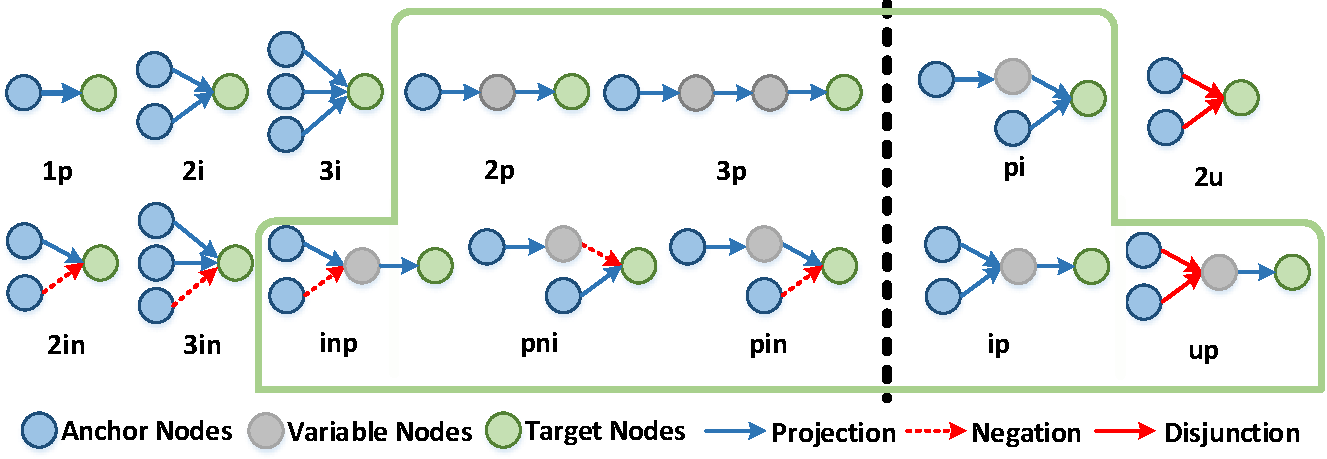
\includegraphics[width=0.45\textwidth]{img/query_pattern.pdf}
    \caption{\textbf{Fourteen queries considered in the experiments.} Where `p', `i', `u', and `n' stand for `projection', `intersection', `union', and `negation', respectively.
    %The numbers 1, 2, 3 indicate the number of relations.
    %The solid green area represents the \emph{existential variable QS (EV-QS)}, while the remaining area denotes the \emph{non-existential variable QS (NV-QS)}. The differences between two areas lie in whether there exist variable nodes in the query sequence.
    }
    \label{fig_2}
\end{figure}
% \vspace{-0.5cm}

\subsubsection*{A.4  Evaluation Metrics}
\label{evaluation_metrics}
The metrics Hit@K and MRR can be defined as follows:
\begin{equation}
\setlength{\abovedisplayskip}{-1pt}
\setlength{\belowdisplayskip}{-3pt}
\textit{Hits}@K(q) = \frac{1}{|A_{q}|}\sum_{v\in A_{q}}{\Phi(\textit{Rank}(v)\leq K)}
\end{equation}
\begin{equation}
\setlength{\belowdisplayskip}{-3pt}
\textit{MRR} = \frac{1}{|A_{q}|}\sum_{v\in A_{q}}{\frac{1}{\textit{Rank}(v)}}
\end{equation}
 $A_{q}$ represents the answer set of \emph{q}, Rank(\emph{v}) denotes as the rank of \emph{v} entity. $\Phi(\cdot)$ is an indicator function, when $x \leq K$, it equals to 1; 0 otherwise. Clearly, higher Hits@K and MRR indicate better prediction performance.

\begin{table*}[htp]
\renewcommand\arraystretch{0.60}
\setlength{\tabcolsep}{1.00em}
\setlength{\belowcaptionskip}{-0.4cm}
\centering
\begin{tabular*}{\linewidth}{@{}cccccccccccc@{}}
\toprule
\multicolumn{1}{c|}{\textbf{Generalization}} & \multicolumn{1}{c|}{\textbf{Method}} & \textbf{1p} & \textbf{2p} & \textbf{3p} & \textbf{2i} & \multicolumn{1}{c|}{\textbf{3i}} & \textbf{pi} & \textbf{ip} & \textbf{2u} & \multicolumn{1}{c|}{\textbf{up}} & \textbf{Avg} \\
\midrule
\multirow{12}*{FB15k}
&GQE   &54.6 	&15.3 	&10.8 	&39.7 	&51.4 	&27.6 	&19.1 	&22.1 	&11.6  &28.0 \\
&\multicolumn{1}{r}{+\textsc{Temp}}   &\textbf{74.9} 	&\textbf{31.4} 	&\textbf{26.0} 	&\textbf{59.3} 	&\textbf{69.4} 	&\textbf{47.3}
&\textbf{35.9} 	&\textbf{47.8} 	&\textbf{27.4} 	&\textbf{46.6} \\
\cmidrule{2-12}
&Q2B   &68.0 	&21.0 	&14.2 	&55.1 	&66.5 	&39.4 	&26.1 	
&35.1  &16.7 	&38.0 \\
&\multicolumn{1}{r}{+\textsc{Temp}}   &\textbf{74.8} 	&\textbf{25.6} 	&\textbf{22.3} 	&\textbf{61.7} 	&\textbf{72.6} 	&\textbf{43.7}
&\textbf{29.0} 	&\textbf{44.1} 	&\textbf{22.5} 	&\textbf{44.0} \\
\cmidrule{2-12}
&\textsc{BetaE}   &65.1 	&25.7 	&24.7 	&55.8 	&66.5 	&43.9 	&28.1 	
&40.1 	&25.2 	&41.6 \\
&\multicolumn{1}{r}{+\textsc{Temp}}   &\textbf{70.3} 	&\textbf{28.9}
&\textbf{25.8} 	&\textbf{58.2} 	&\textbf{68.4}  &\textbf{45.8}
&\textbf{32.2} 	&\textbf{44.3} 	&\textbf{27.3} 	&\textbf{44.6} \\
\cmidrule{2-12}
&\textsc{LogicE}   &72.3 	&29.8 	&26.2 	&56.1 	&66.3 	&42.7 	&32.6 	
&43.4 	&27.5 	&44.1 \\
&\multicolumn{1}{r}{+\textsc{Temp}}   &\textbf{74.9} 	&\textbf{30.9} 	&\textbf{27.3}  &\textbf{58.3} 	&\textbf{68.2} 	&\textbf{43.8}
&\textbf{33.8} 	&\textbf{46.1} 	&\textbf{28.9} 	&\textbf{45.8} \\

\midrule
\multirow{12}*{FB15k-237}
&GQE   &35.0 	&7.2 	&5.3 	&23.3 	&34.6 	&16.5 	&10.7 	
&8.2   &5.7 	&16.3 \\
&\multicolumn{1}{r}{+\textsc{Temp}}   &\textbf{42.9} 	&\textbf{12.3}
&\textbf{10.1} 	&\textbf{34.4} 	&\textbf{47.6} 	&\textbf{26.0}
&\textbf{15.1} 	&\textbf{15.1} 	&\textbf{10.1} 	&\textbf{23.7} \\
\cmidrule{2-12}
&Q2B   &40.6 	&9.4 	&6.8 	&29.5 	&42.3 	&21.2 	&\textbf{12.6} 	
&11.3 	&7.6 	&20.1 \\
&\multicolumn{1}{r}{+\textsc{Temp}}   &\textbf{40.9} 	&\textbf{11.0}
&\textbf{9.2} 	&\textbf{33.7} 	&\textbf{48.2} 	&\textbf{21.4}
&12.3 	&\textbf{12.9} 	&\textbf{9.1} 	&\textbf{22.1}  \\
\cmidrule{2-12}
&\textsc{BetaE}   &39.0 	&10.9 	&10.0 	&28.8 	&42.5 	&22.4 	&12.6 	
&12.4    &9.7 	&20.9 \\
&\multicolumn{1}{r}{+\textsc{Temp}}   &\textbf{39.9} 	&\textbf{11.8}
&\textbf{10.5} 	&\textbf{32.6} 	&\textbf{46.7} 	&\textbf{24.9}
&\textbf{13.6} 	&\textbf{12.5} 	&\textbf{10.2} 	&\textbf{22.5} \\
\cmidrule{2-12}
&\textsc{LogicE}   &41.3 	&11.8 	&10.4 	&31.4 	&43.9 	&23.8 	&14.0 	
&13.4 	&10.2 	&22.3 \\
&\multicolumn{1}{r}{+\textsc{Temp}}   &\textbf{41.9} 	&\textbf{13.0}
&\textbf{11.2} 	&\textbf{32.4} 	&\textbf{45.4} 	&\textbf{25.5} 	
&\textbf{15.2} 	&\textbf{14.6} 	&\textbf{10.9} 	&\textbf{23.3} \\

\midrule
\multirow{12}*{NELL}
&GQE   &32.8 	&11.9 	&9.6 	&27.5 	&35.2 	&18.4 	&14.4 	
&8.5   &8.8 	&18.6 \\
&\multicolumn{1}{r}{+\textsc{Temp}}   &\textbf{57.7} 	&\textbf{17.2}
&\textbf{14.1} 	&\textbf{40.6} 	&\textbf{49.9} 	&\textbf{27.0} 
&\textbf{18.5} 	&\textbf{15.9} 	&\textbf{11.6} 	&\textbf{28.0} \\
\cmidrule{2-12}
&Q2B   &42.2 	&14.0 	&11.2 	&33.3 	&44.5 	&\textbf{22.4} 	&\textbf{16.8}  &11.3  &\textbf{10.3} 	&22.9 \\
&\multicolumn{1}{r}{+\textsc{Temp}}   &\textbf{56.5} 	&\textbf{15.0}
&\textbf{12.9} 	&\textbf{40.8} 	&\textbf{52.0} 	&21.1	
&16.0 	&\textbf{14.2} 	&9.4 	&\textbf{26.4}  \\
\cmidrule{2-12}
&\textsc{BetaE}   &53.0 	&13.0 	&11.4 	&37.6 	&47.5 	&\textbf{24.1} 	&14.3 	
&12.2    &8.5 	&24.6 \\
&\multicolumn{1}{r}{+\textsc{Temp}}   &\textbf{54.1} 	&\textbf{14.2}
&\textbf{12.4} 	&\textbf{38.1} 	&\textbf{48.9} 	&23.9
&\textbf{16.0} 	&\textbf{12.8} 	&\textbf{9.2} 	&\textbf{25.5} \\
\cmidrule{2-12}
&\textsc{LogicE}   &58.3 	&17.7 	&15.4 	&40.5 	&50.4 	&27.3 	&19.2 	
&15.9     &12.7 	&28.6 \\
&\multicolumn{1}{r}{+\textsc{Temp}}   &\textbf{58.4} 	&\textbf{18.1}
&\textbf{14.9} 	&\textbf{40.7} 	&\textbf{50.6} 	&\textbf{27.9}
&\textbf{19.1} 	&\textbf{16.7} 	&\textbf{12.8} 	&\textbf{28.8} \\

\bottomrule
\end{tabular*}
\caption{Detailed MRR results on the \textsc{BetaE}'s datasets testing generalization.}
\label{table_7}
\end{table*}

\begin{table*}[htp]
\renewcommand\arraystretch{0.60}
\setlength{\tabcolsep}{0.90em}
\setlength{\belowcaptionskip}{-0.4cm}
\small
\centering
\begin{tabular*}{\linewidth}{@{}cccccccccccccc@{}}
\toprule
\multicolumn{1}{c|}{\textbf{Datasets}} & \multicolumn{1}{c|}{\textbf{Methods}} & \textbf{TER} & \textbf{TRR} & \textbf{1p} & \textbf{2p} & \textbf{3p} & \textbf{2i} & \multicolumn{1}{c|}{\textbf{3i}} & \textbf{pi} & \textbf{ip} & \textbf{2u} & \multicolumn{1}{c|}{\textbf{up}} & \textbf{Avg} \\
\midrule
\multirow{12}*{FB15k}
&\multirow{5}*{GQE}
&\tiny \XSolidBold  &\tiny \XSolidBold  &55.1 	&30.7 	&22.5 	&38.6 	&49.3 	&24.9 	&14.6 	&34.3 	&25.1 	&32.8 \\
&   &\tiny \CheckmarkBold  & \tiny \XSolidBold   &65.3 	&38.1 	&29.4 	
&52.1 	&64.3 	&35.5 	&17.9 	&44.6 	&31.4 	&42.1 \\
&   &\tiny \XSolidBold  &\tiny \CheckmarkBold  &74.2 	&49.8 	&\textbf{42.0}  &56.2 	&66.6 	&44.3 	&27.3 	&59.1 	&\textbf{37.7} 	&50.8 \\
&   &\tiny \CheckmarkBold  &\tiny \CheckmarkBold  &\textbf{75.2} 	
&\textbf{50.4} 	&\textbf{42.0}  &\textbf{56.9} 	&\textbf{67.1} 	
&\textbf{44.5} 	&\textbf{28.2} 	&\textbf{59.5} 	&34.0 	&\textbf{50.9} \\ \cmidrule{2-14}
&\multirow{5}*{Q2B}
&\tiny \XSolidBold  &\tiny \XSolidBold  &68.3 	&39.0 	&28.5 	&52.2 	&64.0 	&37.4 	&20.1 	&50.6 	&30.1 	&43.4 \\
&   &\tiny \CheckmarkBold  & \tiny \XSolidBold   &72.4 	&37.3 	&28.6 	&55.7 	&67.7 	&36.0 	&17.4 	&57.1 	&26.3 	&44.3 \\
&   &\tiny \XSolidBold  &\tiny \CheckmarkBold  &69.9 	&\textbf{46.1} 	&\textbf{38.8} 	&56.2 	&68.6 	&41.8 	&\textbf{25.6} 	&52.7 	&\textbf{29.3}  &47.7  \\
&   &\tiny \CheckmarkBold  &\tiny \CheckmarkBold  &\textbf{75.6} 	&45.5	&38.4 	&\textbf{60.0} 	&\textbf{71.0} 	&\textbf{43.1} 	&23.6 	&\textbf{62.7} 	&27.4 	&\textbf{49.7}  \\
\midrule

\multirow{12}*{FB15k-237}
&\multirow{5}*{GQE}
&\tiny \XSolidBold  &\tiny \XSolidBold  &35.0 	&19.2 	&14.4 	&22.1 	&31.4 	&14.5 	&8.8 	&14.8 	&14.5 	&19.4 \\
&   &\tiny \CheckmarkBold  & \tiny \XSolidBold  &40.3 	&22.2 	&17.5 	&27.0 	&38.3 	&17.3 	&9.9 	&21.1 	&18.1 	&23.5 \\
&   &\tiny \XSolidBold  &\tiny \CheckmarkBold   &\textbf{43.9} 	&26.8 	&22.5 	&28.2 	&37.6 	&20.4 	&11.9 	&24.9 	&\textbf{20.9} 	&26.3 \\
&   &\tiny \CheckmarkBold  &\tiny \CheckmarkBold  &43.0 &\textbf{27.7} 	&\textbf{23.4} 	&\textbf{32.6} 	&\textbf{44.4} 	&\textbf{23.4} 	&\textbf{13.2} 	&\textbf{26.5} 	&20.0 	&\textbf{28.2} \\
\cmidrule{2-14}
&\multirow{5}*{Q2B}
&\tiny \XSolidBold  &\tiny \XSolidBold  &40.7 	&23.1 	&18.1 	&27.9 	&38.9 	&19.2 	&10.9 	&21.1 	&\textbf{17.8} 	&24.2 \\
&   &\tiny \CheckmarkBold  & \tiny \XSolidBold   &42.1 	&23.1 	&17.6 	&29.6 	&41.3 	&18.1 	&9.9 	&22.7 	&17.7 	 &24.7 \\
&   &\tiny \XSolidBold  &\tiny \CheckmarkBold    &\textbf{42.2} 	&\textbf{26.0} 	&21.6 	&29.6 	&42.0 	&18.6 	&\textbf{12.2} 	&22.1 	&\textbf{17.8} 	 &25.8  \\
&   &\tiny \CheckmarkBold  &\tiny \CheckmarkBold &41.2 	&25.8 	&\textbf{21.9} 	&\textbf{33.1} 	&\textbf{45.0} 	&\textbf{21.0} 	&11.4 	&\textbf{24.4} 	&17.7  	 &\textbf{26.8}  \\
\midrule

\multirow{12}*{NELL}
&\multirow{5}*{GQE}
&\tiny \XSolidBold  &\tiny \XSolidBold  &31.3 	&18.2 	&16.8 	&22.4 	&30.4 	&15.8 	&10.0 	&16.8 	&12.1 	&19.3 \\
&   &\tiny \CheckmarkBold  & \tiny \XSolidBold  &51.2 	&21.9 	&21.7 	&28.5 	&40.6 	&17.5 	&9.2 	&35.1 	&15.6 	&26.8 \\
&   &\tiny \XSolidBold  &\tiny \CheckmarkBold   &55.5 	&31.8 	&31.7 	&33.6 	&46.1 	&23.0 	&14.1 	&38.9 	&24.4 	&33.2 \\
&   &\tiny \CheckmarkBold  &\tiny \CheckmarkBold  &\textbf{56.7} &\textbf{33.6} 	&\textbf{32.4} 	&\textbf{35.5} 	&\textbf{47.2} 	&\textbf{23.6} 	&\textbf{14.8} 	&\textbf{41.6} 	&\textbf{24.8} 	&\textbf{34.5} \\
\cmidrule{2-14}
&\multirow{5}*{Q2B}
&\tiny \XSolidBold  &\tiny \XSolidBold  &41.8 	&23.1 	&21.2 	&28.9 	&41.7 	&\textbf{19.7} 	&12.2 	&26.9 	&15.5 	&25.7 \\
&   &\tiny \CheckmarkBold  & \tiny \XSolidBold   &54.4 	&22.9 	&23.0 	&33.7 	&47.4 	&15.9 	&10.1 	&38.7 	&15.8 	&29.1 \\
&   &\tiny \XSolidBold  &\tiny \CheckmarkBold    &55.9 	&31.1 	&\textbf{31.3} 	&34.8 	&48.9 	&19.4 	&\textbf{14.0} 	&41.2 	&23.6 	&33.4  \\
&   &\tiny \CheckmarkBold  &\tiny \CheckmarkBold &\textbf{57.1} 	&\textbf{31.9} 	&\textbf{31.3} 	&\textbf{36.6} 	&\textbf{49.5} 	&19.4 	&13.5 	&\textbf{41.7} 	&\textbf{23.8} 	&\textbf{33.9}  \\

\bottomrule
\end{tabular*}
\caption{Detailed MRR results on the Q2B datasets with TER or TRR.}
\label{table_8}
\end{table*}


\subsection*{B  Design Alternatives}
\label{section_design_alternatives}
In our ablation experiments, we test \textsc{Temp} with the following alternative models. In particular, when aggregating the type of an entity, we propose two alternatives for aggregator, instead of the highway aggregator in Eqs. (\ref{highway_agg_1}), (\ref{highway_agg_2}), and (\ref{highway_agg_3}). \\
\vspace{-0.4cm}
\paragraph{Mean aggregator.}
\begin{equation}
\setlength{\abovedisplayskip}{-3pt}
\setlength{\belowdisplayskip}{-3pt}
\widetilde{\mathcal{H}_{s}^{K}} = \frac{1}{n}\sum_{i} \mathcal{H}_{s_{i}}^{K}
\end{equation}
Here, the mean operation does not require a loop operation, so the value of \emph{K} is 0. $\mathcal{H}_{s_{i}}^{K}\in\mathbb{R}^{d\times 1}$ represents the \emph{i-th} component of the vector $\mathcal{H}_{s}^{K}\in\mathbb{R}^{d\times n}$. \\
\vspace{-0.4cm}
\paragraph{Max  aggregator.}
\begin{equation}
\setlength{\abovedisplayskip}{-3pt}
\setlength{\belowdisplayskip}{-1pt}
\widetilde{\mathcal{H}_{s}^{K}} = \textit{Max}(\mathcal{H}_{s_{i}}^{K})
\end{equation}
%\vspace{-0.5cm}
$\textit{Max}(\cdot)$ represents the element-wise maximum operation among the entity's type information. \emph{K} also takes 0.\\
\vspace{-0.4cm}
\paragraph{Concatenation-based intersection.} Inspired by ~\cite{liu2016learning} and ~\cite{reimers2019sentence}, we apply an interactive concatenation to pair of the representations $\mathcal{G}^{er}$ and $\mathcal{G}^{es}$ in Eqs.(\ref{dcmn_1}) and (\ref{dcmn_2}), and then perform a linear layer operation. The interactive concatenation can be specified as:
\begin{equation}
\setlength{\abovedisplayskip}{-2pt}
\setlength{\belowdisplayskip}{-2pt}
\widetilde{\mathcal{G}^{e}} = W[\mathcal{G}^{er}, \mathcal{G}^{es}, \mathcal{G}^{er}+\mathcal{G}^{es}, \mathcal{G}^{er}\times\mathcal{G}^{es}] + b,
\end{equation}
where $+$ and $\times$ represent the element-wise addition and multiplication between two matrices $\mathcal{G}^{er}$ and $\mathcal{G}^{es}$, respectively. $[\cdot, \cdot, \cdot, \cdot]$ is used to concatenate the vector in row level.

% \begin{figure}[htp]
% \begin{minipage}[t]{0.45\linewidth}
% \centering
% 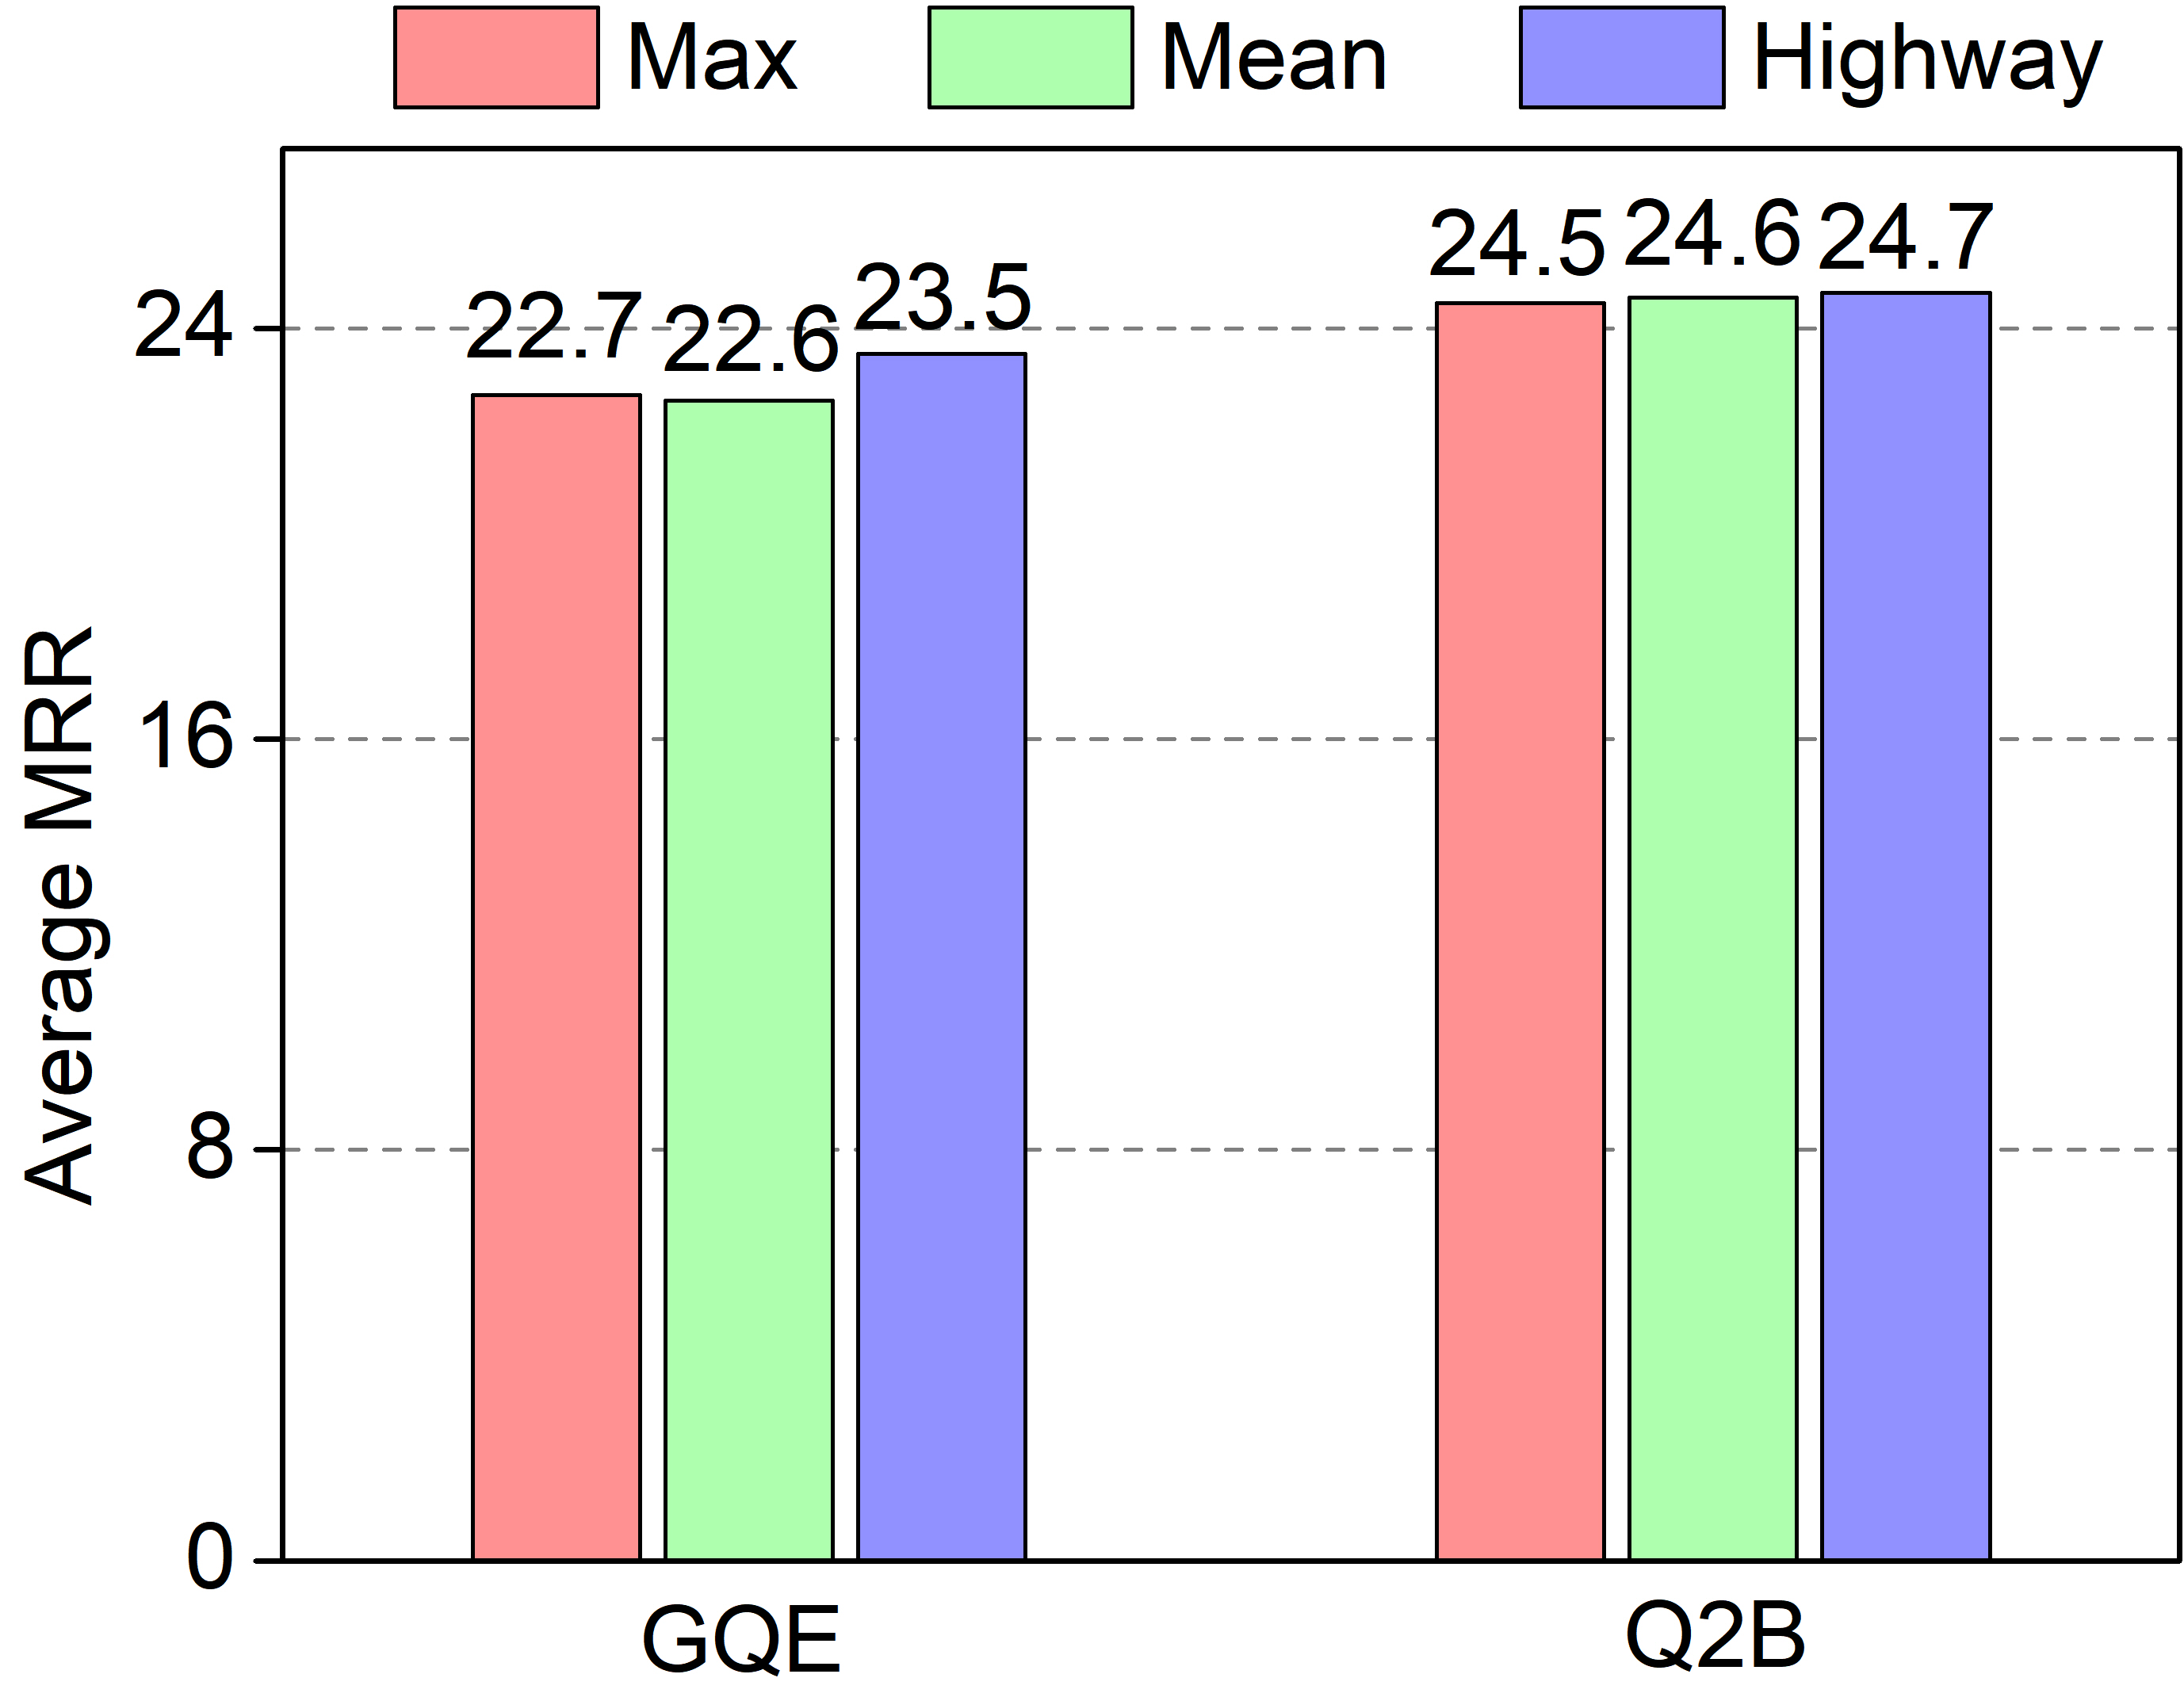
\includegraphics[height=3.5cm,width=4cm]{img/entity_ablation.jpg}
% \caption{MRR results with different entity type aggregators.}
% \label{Figure_4}
% \end{minipage}%
% \hspace{8mm}
% \begin{minipage}[t]{0.45\linewidth}
% \centering
% 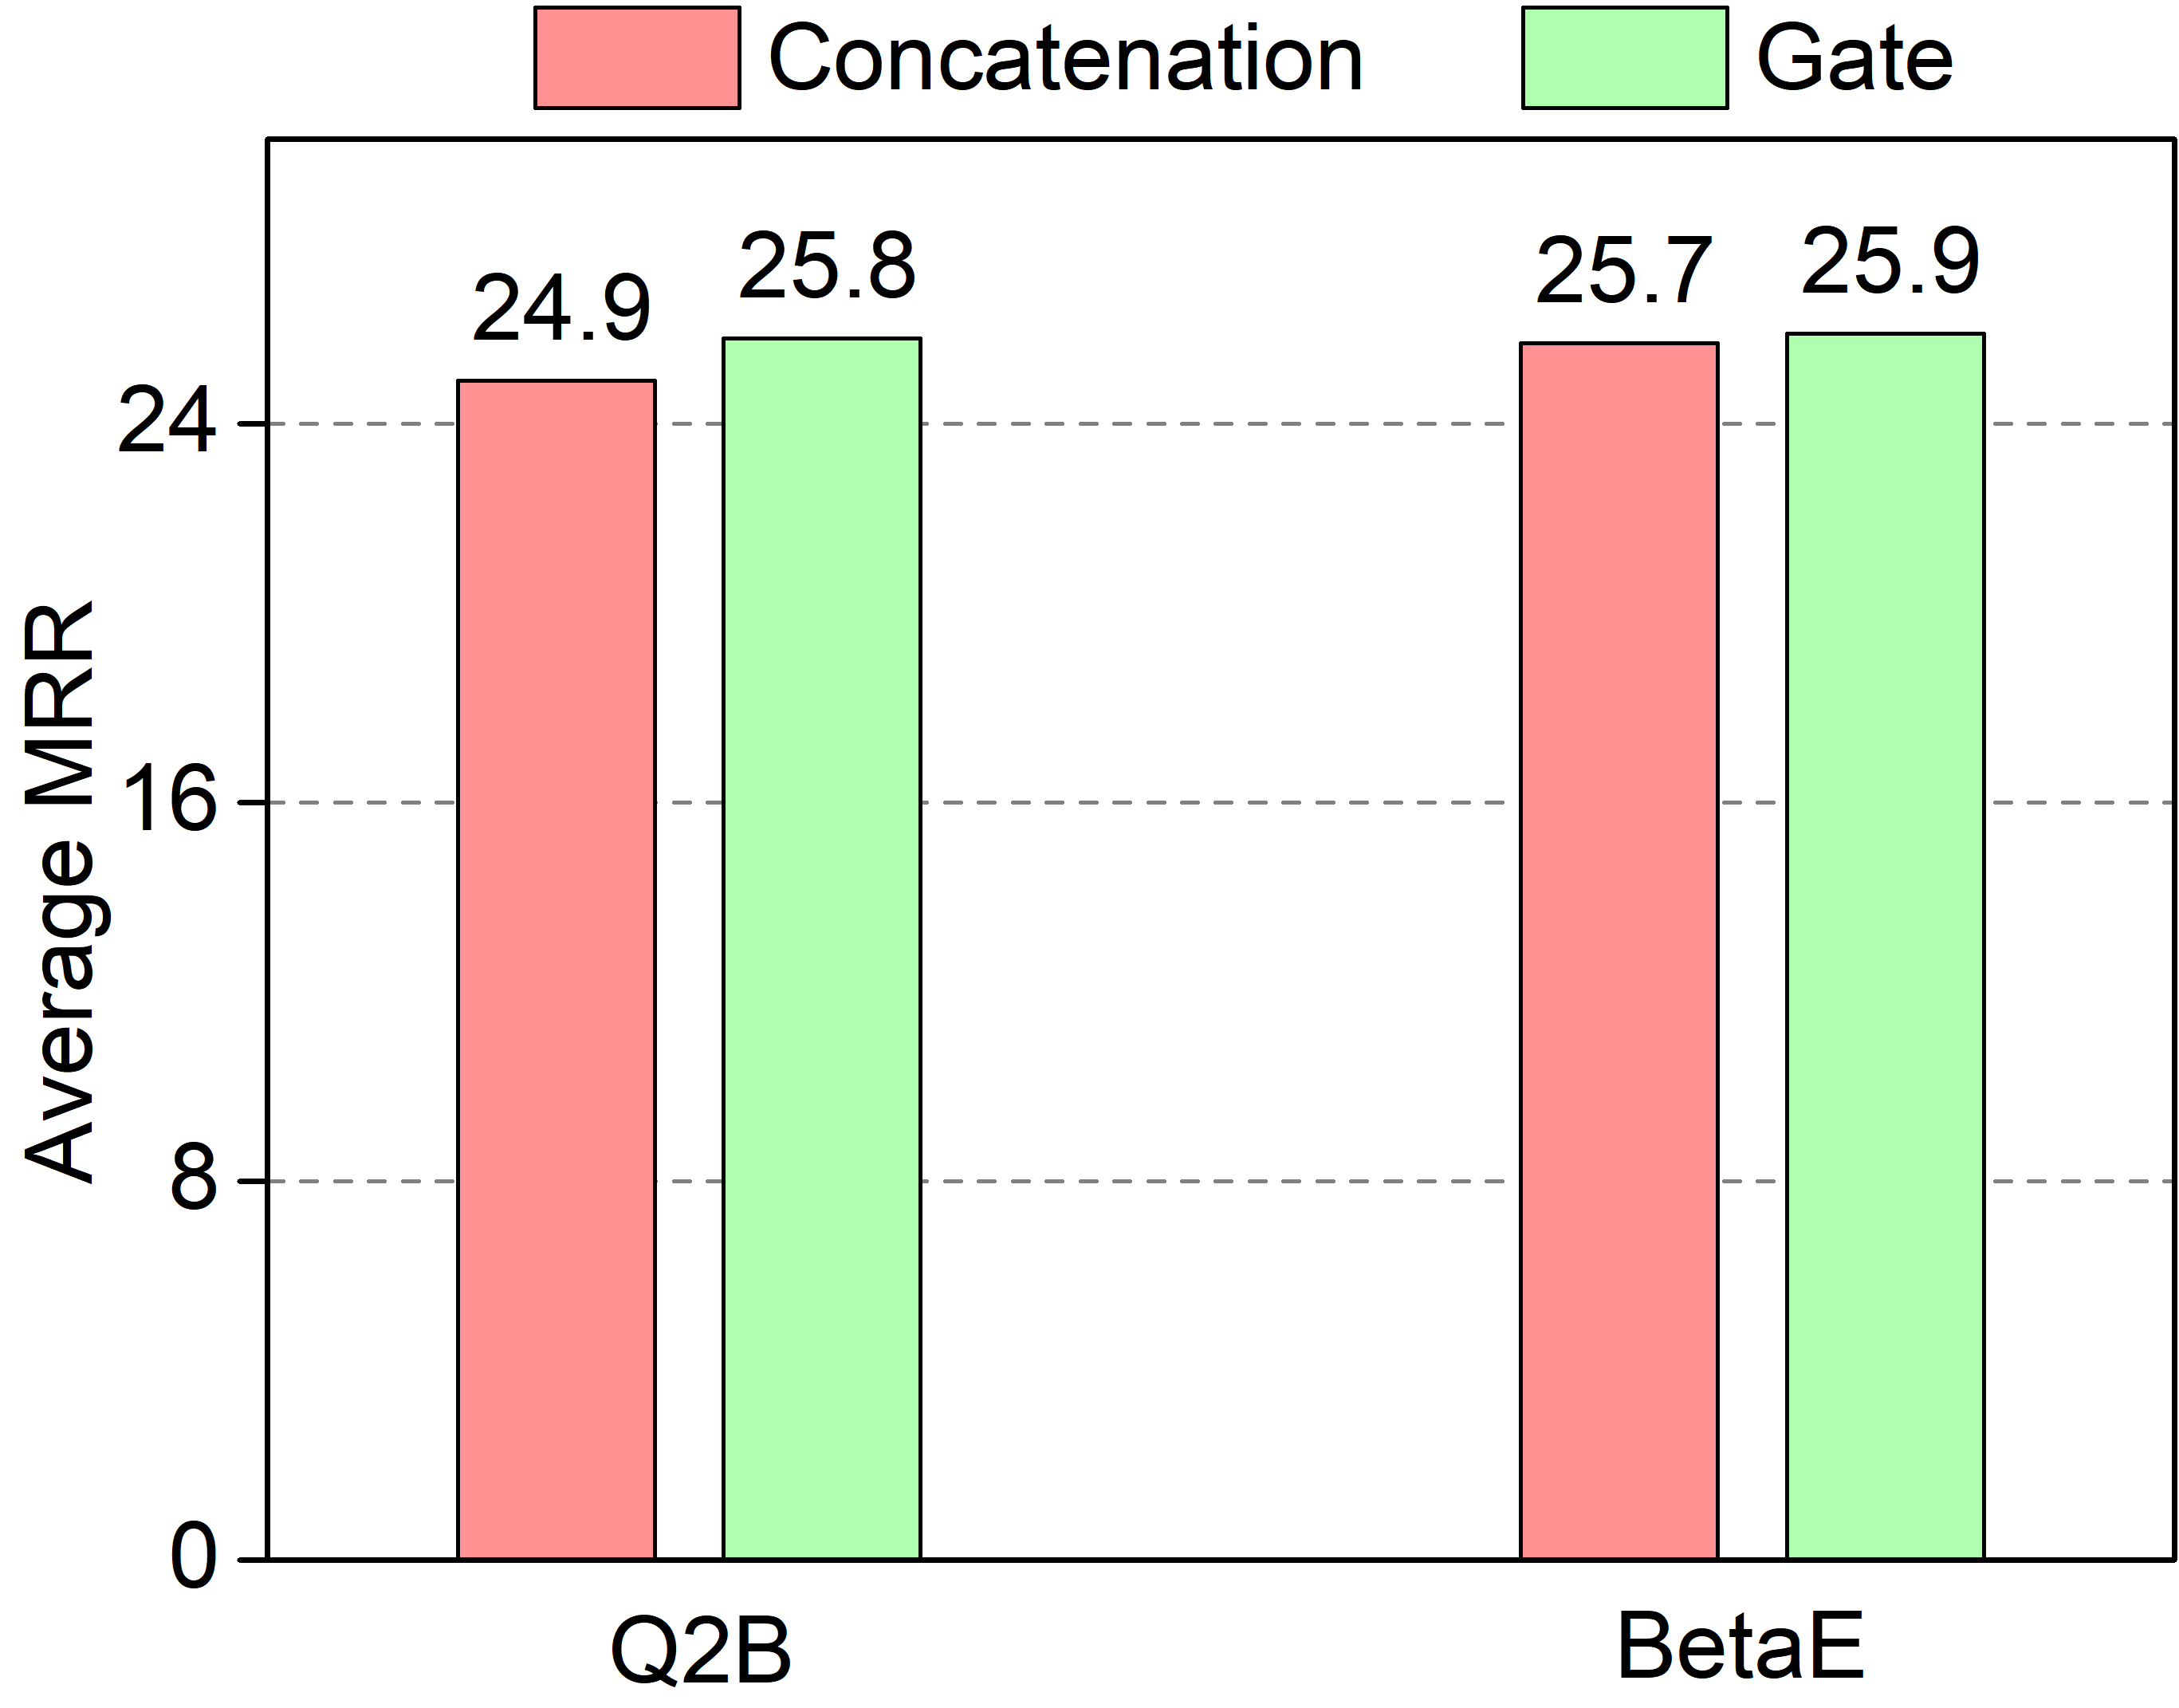
\includegraphics[height=3.5cm,width=4cm]{img/relation_ablation.jpg}
% \caption{MRR results with different relation type aggregators.}
% \label{figure_5}
% \end{minipage}
% \end{figure}

% \begin{figure*}[htb]
%     \centering
%     \begin{minipage}[t]{0.45\textwidth}
%         \centering
%         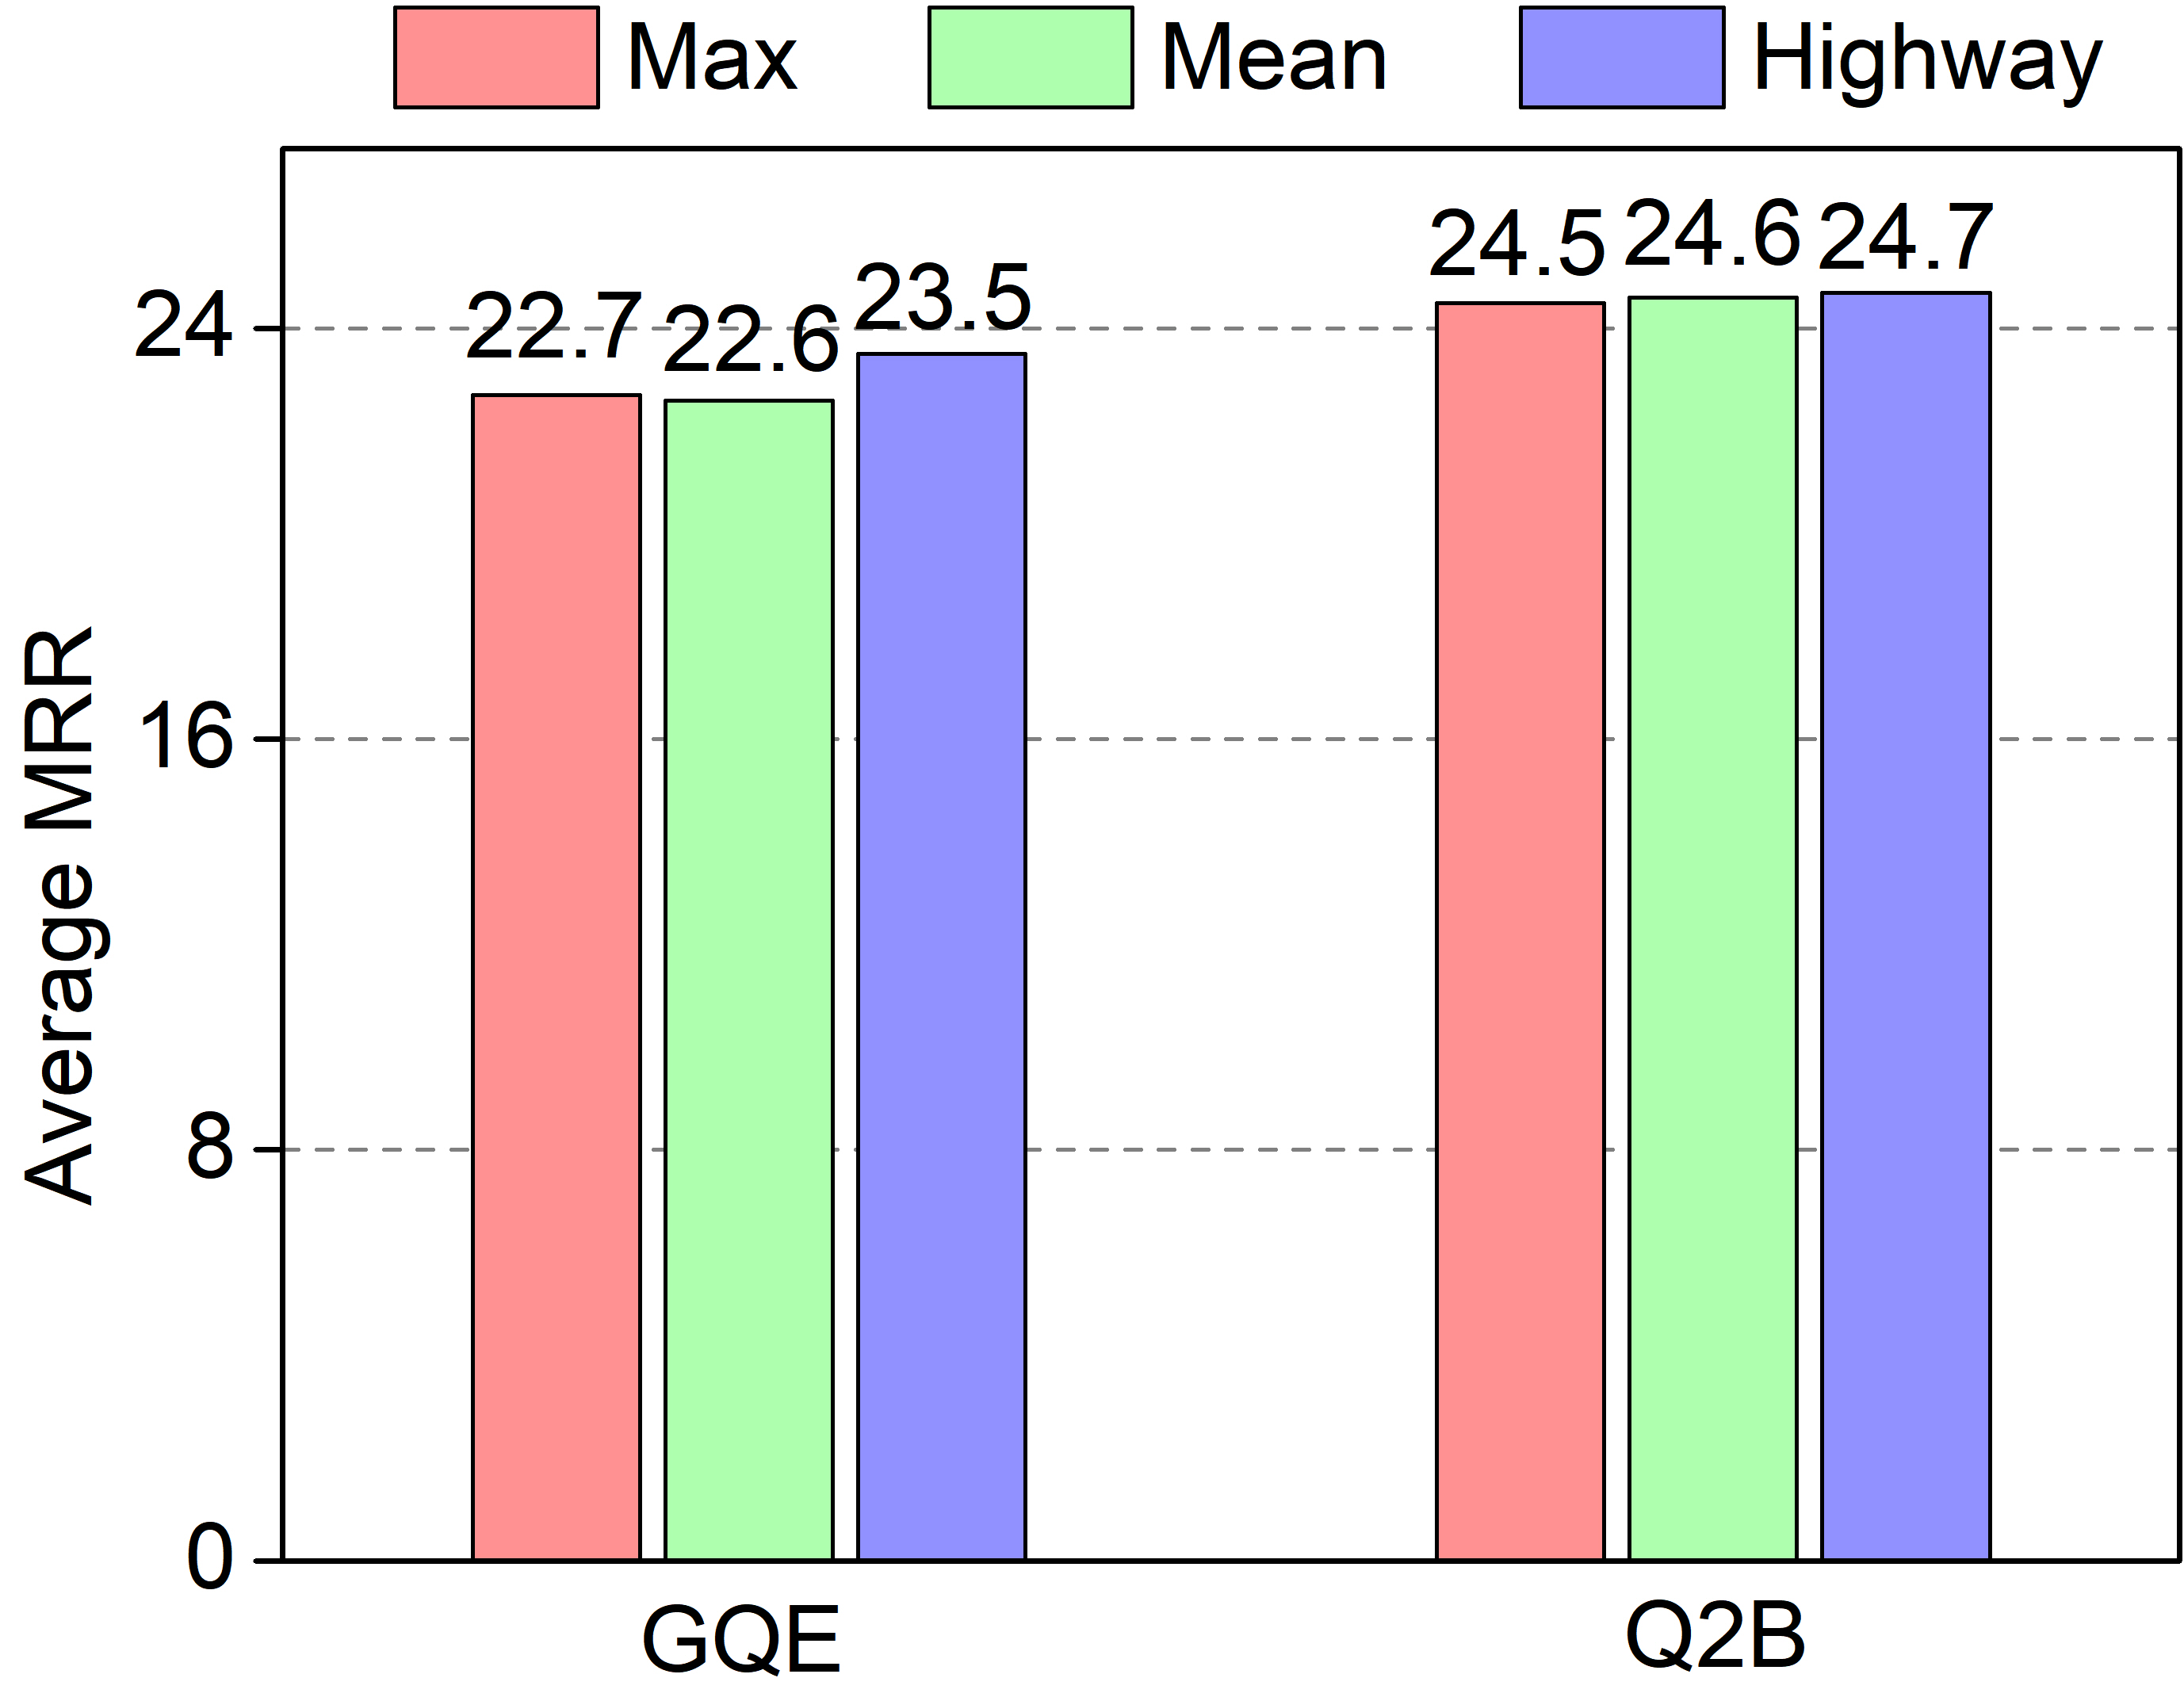
\includegraphics[width=0.9\textwidth]{img/entity_ablation.jpg} % first figure itself
%         \caption{MRR results with different entity type aggregators.}
%         \label{Figure_4}
%     \end{minipage}\hfill
%     \begin{minipage}[t]{0.45\textwidth}
%         \centering
%         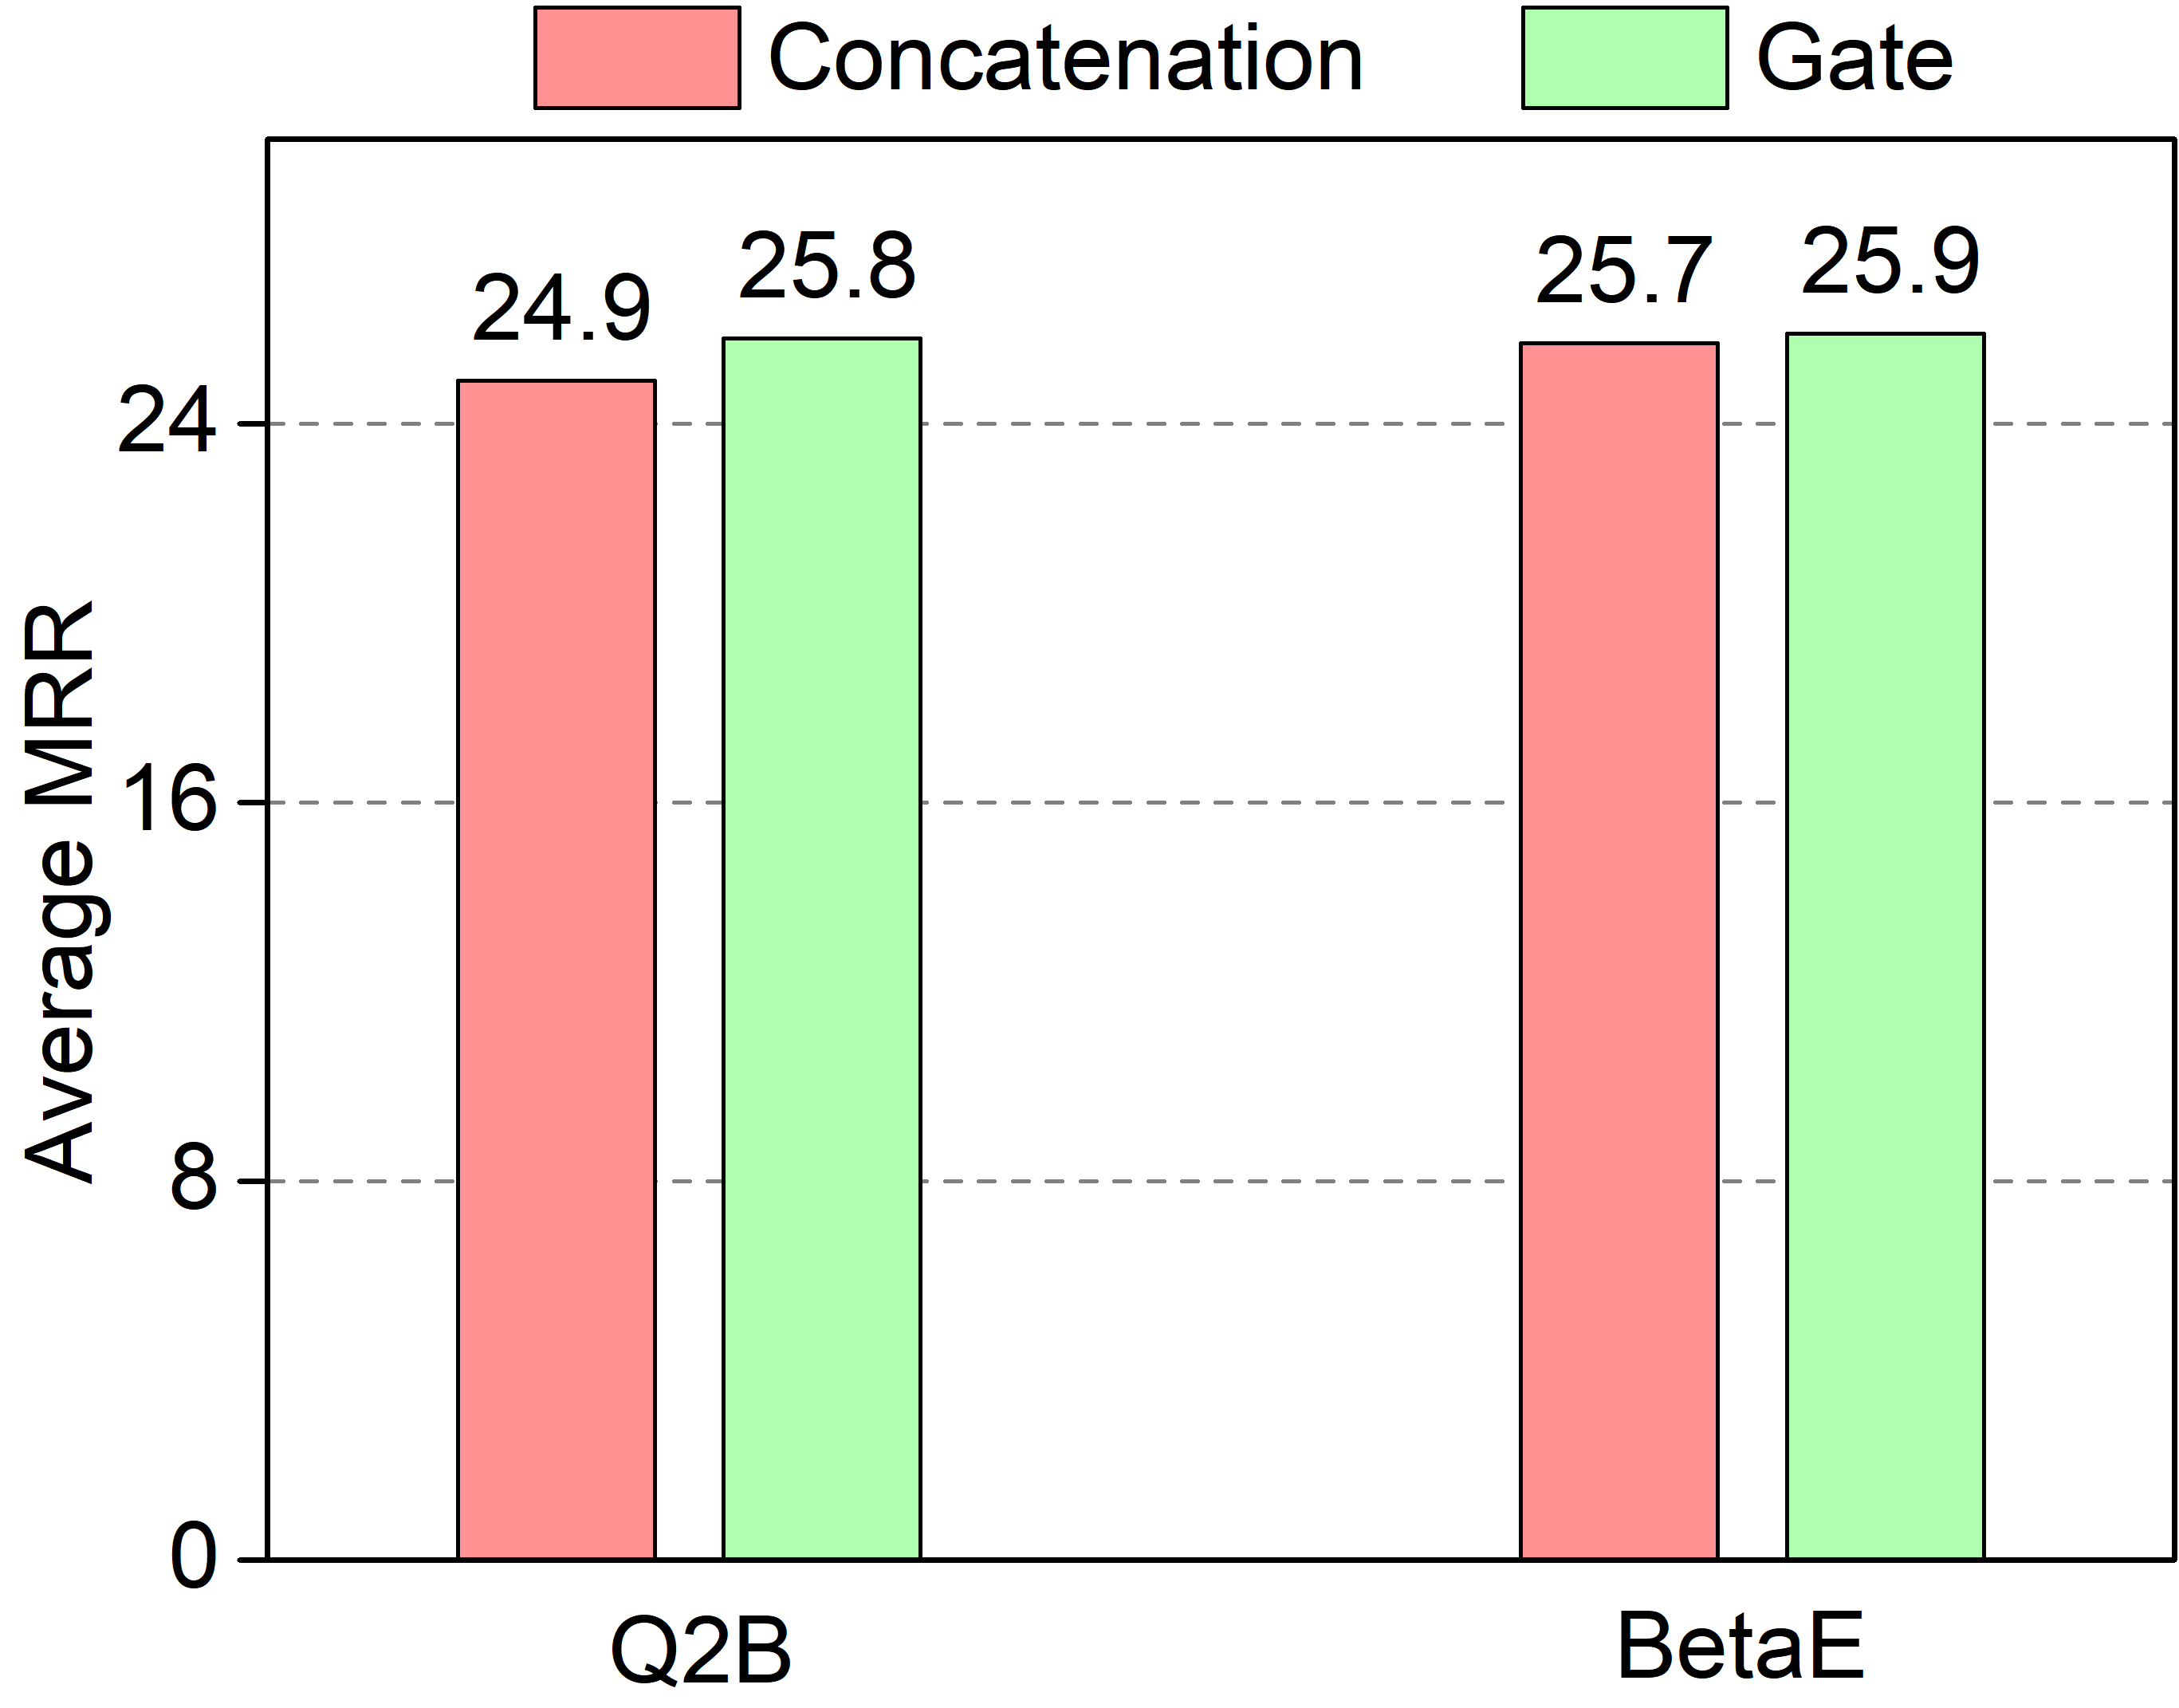
\includegraphics[width=0.9\textwidth]{img/relation_ablation.jpg} % second figure itself
%         \caption{MRR results with different relation type aggregators.}
%         \label{figure_5}
%     \end{minipage}
% \end{figure*}

\subsection*{C  Additional Results}
%In this section, we discuss more experimental results that are not included in the main part of the paper.  
%\subsubsection*{C.1  Results with Different Entity Type Aggregators and Relation Type Aggregators.}
\begin{enumerate}
\item Table \ref{table_7} shows  detailed MRR results on the \textsc{BetaE} datasets, testing the generalization ability.

\item Table \ref{table_8} shows  detailed MRR results on the Q2B datasets with TER or TRR used separately  or together.

\item Table \ref{table_9} shows  detailed Hits@3 results on the Q2B datasets about the generalization and deductive reasoning ability.

% \item 
% Figure \ref{Figure_4} and~ \ref{figure_5} show the results on considering different entity type aggregators and relation type aggregators as described in \nameref{section_design_alternatives} on the Q2B's FB15k-237 datasets,
% respectively.  
%\vspace{-0.2cm}
\end{enumerate}


% \subsubsection*{C.2  Detailed MRR Results on the \textsc{BetaE} Datasets Testing Generalization }
% Table \ref{table_6} shows the detailed MRR results on the \textsc{BetaE} datasets to test the generalization ability.
% \subsubsection*{C.3  Detailed MRR Results with TER or TRR}
% Table \ref{table_7} shows the detailed MRR results on the Q2B datasets with TER or TRR join alone or at the same time.
% \subsubsection*{C.4  Detailed Results with Generalization and Deductive Reasoning Ability}
% Table \ref{table_8} shows the detailed Hits@3 results on the Q2B datasets about the generalization and deductive reasoning ability.
%\vspace{-0.2cm}

\begin{table*}[!htp]
\renewcommand\arraystretch{0.60}
\setlength{\tabcolsep}{0.95em}
\centering
\begin{tabular*}{\linewidth}{@{}cccccccccccc@{}}
\toprule
\textbf{Generalization} & \multicolumn{1}{c|}{\textbf{Method}} & \textbf{1p} & \textbf{2p} & \textbf{3p} & \textbf{2i} & \multicolumn{1}{c|}{\textbf{3i}} & \textbf{pi} & \textbf{ip} & \textbf{2u} & \multicolumn{1}{c|}{\textbf{up}} & \textbf{Avg} \\
\midrule
\multirow{12}*{FB15k}
&GQE   &71.7 	&36.1 	&25.9 	&47.5 	&60.8 	&30.0 	&15.8 	&45.2 	&28.1 	&40.1 \\
&\multicolumn{1}{r}{+\textsc{Temp}}   &\textbf{83.0} 	&\textbf{54.6} 	&\textbf{46.0} 	&\textbf{64.1} 	&\textbf{74.8} 	&\textbf{50.0} 	&\textbf{30.8} 	&\textbf{68.7}
&\textbf{37.3} 	&\textbf{56.6} \\
\cmidrule{2-12}
&Q2B   &82.1 	&43.0 	&31.7 	&62.7 	&74.5 	&44.4 	&22.4 	&66.7 	&\textbf{33.5} 	&51.2 \\
&\multicolumn{1}{r}{+\textsc{Temp}}   &\textbf{84.0} 	&\textbf{49.8} 	&\textbf{42.2} 	&\textbf{67.4} 	&\textbf{77.9} 	&\textbf{48.3} 	&\textbf{26.1} 	&\textbf{72.7}
&30.0 	&\textbf{55.4} \\
\cmidrule{2-12}
&\textsc{BetaE}   &75.0 	&45.1 	&40.0 	&62.2 	&\textbf{75.4} 	&47.1 	&22.3 	&58.9 	&29.6 	&50.6 \\
&\multicolumn{1}{r}{+\textsc{Temp}}   &\textbf{79.5} 	&\textbf{50.2} 	&\textbf{44.3} 	&\textbf{63.7} 	&74.4 	&\textbf{48.8} 	&\textbf{27.4} 	&\textbf{64.5}
&\textbf{30.0} 	&\textbf{53.6} \\
\cmidrule{2-12}
&\textsc{LogicE}   &80.5 	&50.5 	&45.8 	&62.2 	&72.5 	&47.5 	&28.3 	&63.9 	&36.8 	&54.2 \\
&\multicolumn{1}{r}{+\textsc{Temp}}   &\textbf{83.2} 	&\textbf{51.5} 	&\textbf{46.4} 	&\textbf{64.0} 	&\textbf{73.8} 	&\textbf{47.8} 	&\textbf{28.6} 	&\textbf{69.0}
&\textbf{36.9} 	&\textbf{55.7} \\
\midrule

\multirow{12}*{FB15k-237}
&GQE   &41.3 	&21.5 	&15.2 	&26.5 	&38.5 	&16.7 	&8.8 	&17.1 	&15.8 	&22.4 \\
&\multicolumn{1}{r}{+\textsc{Temp}}   &\textbf{47.6} 	&\textbf{29.6} 	&\textbf{24.7} 	&\textbf{36.3} 	&\textbf{48.4} 	&\textbf{25.5} 	&\textbf{13.4} 	&\textbf{30.2}
&\textbf{21.0} 	&\textbf{30.7} \\
\cmidrule{2-12}
&Q2B   &\textbf{47.1} 	&24.9 	&19.4 	&33.2 	&46.4 	&21.8 	&11.3 	&25.3 	&\textbf{19.3} 	&27.6 \\
&\multicolumn{1}{r}{+\textsc{Temp}}   &45.7  	&\textbf{27.8} 	&\textbf{23.4} 	&\textbf{36.9} 	&\textbf{49.6} 	&\textbf{22.9} 	&\textbf{11.7} 	&\textbf{27.6}
&18.9 	&\textbf{29.4} \\
\cmidrule{2-12}
&\textsc{BetaE}   &42.6 	&25.4 	&21.6 	&30.2 	&43.3 	&20.7 	&9.2 	&24.2 	&\textbf{18.3} 	&26.2 \\
&\multicolumn{1}{r}{+\textsc{Temp}}   &\textbf{43.3} 	&\textbf{27.2} 	&\textbf{22.7} 	&\textbf{35.3} 	&\textbf{47.5} 	&\textbf{24.3} 	&\textbf{10.6} 	&\textbf{26.7}
&18.2 	&\textbf{28.4} \\
\cmidrule{2-12}
&\textsc{LogicE}   &45.6 	&27.8 	&24.1 	&34.7 	&46.5 	&23.5 	&12.0 	&27.1 	&20.8 	&29.1 \\
&\multicolumn{1}{r}{+\textsc{Temp}}   &\textbf{46.6} 	&\textbf{29.2} 	&\textbf{25.0} 	&\textbf{35.8} 	&\textbf{47.9} 	&\textbf{24.9} 	&\textbf{13.5} 	&\textbf{28.7}
&\textbf{21.0} 	&\textbf{30.3} \\
\midrule

\multirow{12}*{NELL}
&GQE   &42.7 	&21.6 	&19.3 	&27.0 	&37.4 	&17.7 	&10.3 	&21.7 	&13.4 	&23.5 \\
&\multicolumn{1}{r}{+\textsc{Temp}}   &\textbf{62.5} 	&\textbf{36.6} 	&\textbf{35.2} 	&\textbf{40.2} 	&\textbf{52.6} 	&\textbf{25.6} 	&\textbf{15.8} 	&\textbf{48.2}  &\textbf{27.4} 	&\textbf{38.2} \\
\cmidrule{2-12}
&Q2B   &56.2 	&27.1 	&24.1 	&34.7 	&49.2 	&\textbf{21.8} 	&12.7 	&37.5 	&16.5  &31.1 \\
&\multicolumn{1}{r}{+\textsc{Temp}}   &\textbf{62.5}  	&\textbf{34.3} 	&\textbf{34.2} 	&\textbf{41.0} 	&\textbf{55.2} 	&20.9 	&\textbf{14.1} 	&\textbf{47.7}  &\textbf{26.2} 	&\textbf{37.3} \\
\cmidrule{2-12}
&\textsc{BetaE}   &58.4 	&29.1 	&30.7 	&35.2 	&48.4 	&22.5 	&10.5 &\textbf{44.5} 	&\textbf{21.2} 	&33.4 \\
&\multicolumn{1}{r}{+\textsc{Temp}}   &\textbf{58.7} 	&\textbf{31.7} 	&\textbf{32.7} 	&\textbf{37.3} 	&\textbf{51.3} 	&\textbf{22.8} 	
&\textbf{11.7} 	&43.7   &20.6 	&\textbf{34.5} \\
\cmidrule{2-12}
&\textsc{LogicE}   &\textbf{64.3} 	&35.9 	&\textbf{36.0} 	&41.1 	&54.8 	
&\textbf{26.8} 	&14.7
&51.0 	&27.6 	&\textbf{39.1} \\
&\multicolumn{1}{r}{+\textsc{Temp}}   &\textbf{64.3} 	&\textbf{36.2} 	&35.9 	&\textbf{41.2} 	&\textbf{54.9} 	&25.4 	&\textbf{15.5} 	&\textbf{51.1}  &\textbf{27.9} 	&\textbf{39.1} \\

\midrule
\textbf{Deductive Reasoning} & \multicolumn{1}{c|}{\textbf{Method}} & \textbf{1p} & \textbf{2p} & \textbf{3p} & \textbf{2i} & \multicolumn{1}{c|}{\textbf{3i}} & \textbf{pi} & \textbf{ip} & \textbf{2u} & \multicolumn{1}{c|}{\textbf{up}} & \textbf{Avg} \\
\midrule
\multirow{12}*{FB15k}
&GQE   &73.8 	&40.5 	&32.1 	&49.8 	&64.7 	&36.1 	&18.9 	&47.2 	&30.4 	&43.7 \\
&\multicolumn{1}{r}{+\textsc{Temp}}   &\textbf{92.8} 	&\textbf{71.5} 	&\textbf{62.0} 	&\textbf{74.6} 	&\textbf{83.8} 	&\textbf{64.4} 	&\textbf{48.0} 	&\textbf{85.5}  &\textbf{60.0} 	&\textbf{71.4} \\
\cmidrule{2-12}
&Q2B   &68.0 	&39.4 	&32.7 	&48.5 	&65.3 	&32.9 	&16.2 	&61.4
&28.9  &43.7 \\
&\multicolumn{1}{r}{+\textsc{Temp}}   &\textbf{92.8} 	&\textbf{67.1} 	&\textbf{57.3} 	&\textbf{79.2} 	&\textbf{87.6} 	&\textbf{62.8} 	&\textbf{39.8} 	&\textbf{87.3}  &\textbf{52.4} 	&\textbf{69.6} \\
\cmidrule{2-12}
&\textsc{BetaE}   &83.2 	&57.3 	&51.0 	&\textbf{71.1} 	&\textbf{81.4} 	
&\textbf{56.9} 	&32.7 	&70.4 	&41.0 	&\textbf{60.6} \\
&\multicolumn{1}{r}{+\textsc{Temp}}   &\textbf{84.0} 	&\textbf{58.8} 	&\textbf{51.8} 	&68.7 	&78.4 	&55.6 	&\textbf{34.8} 	&\textbf{71.6}
&\textbf{41.9} 	&\textbf{60.6} \\
\cmidrule{2-12}
&\textsc{LogicE}   &88.4 	&64.0 	&57.9 	&70.8 	&80.6 	&59.0 	&41.0 	&76.6 &51.0 	  &65.5 \\
&\multicolumn{1}{r}{+\textsc{Temp}}   &\textbf{91.0} 	&\textbf{64.7} 	&\textbf{58.7} 	&\textbf{72.3} 	&\textbf{81.4} 	&\textbf{60.5} 	&\textbf{42.2} 	&\textbf{81.2}  &\textbf{51.5} 	&\textbf{67.1} \\

\midrule
\multirow{12}*{FB15k-237}
&GQE   &56.4 	&30.1 	&24.5 	&35.9 	&51.2 	&25.1 	&13.0 	&25.8 	&22.0  &31.6 \\
&\multicolumn{1}{r}{+\textsc{Temp}}   &\textbf{76.3} 	&\textbf{48.6} 	&\textbf{39.0} 	&\textbf{49.7} 	&\textbf{60.4} 	&\textbf{36.9} 	&\textbf{22.1} 	&\textbf{59.0}  &\textbf{36.3} 	&\textbf{47.6} \\
\cmidrule{2-12}
&Q2B   &58.5 	&34.3 	&28.1 	&44.7 	&62.1 	&23.9 	&11.7 	
&40.5  &22.0    &36.2 \\
&\multicolumn{1}{r}{+\textsc{Temp}}   &\textbf{87.2} 	&\textbf{59.6} 	&\textbf{47.9} 	&\textbf{67.2} 	&\textbf{72.7} 	&\textbf{49.1} 	&\textbf{29.8} 	&\textbf{78.6}  &\textbf{43.4} 	&\textbf{59.5} \\
\cmidrule{2-12}
&\textsc{BetaE}   &77.9 	&52.6 	&44.5 	&59.0 	&67.8 	&42.2 	&23.5 	&63.7 	&35.1 	 &51.8 \\
&\multicolumn{1}{r}{+\textsc{Temp}}   &\textbf{84.7} 	&\textbf{58.3} 	&\textbf{49.4} 	&\textbf{62.3} 	&\textbf{68.8} 	&\textbf{45.3} 	&\textbf{28.5} 	&\textbf{74.5}  &\textbf{41.4} 	&\textbf{57.0} \\
\cmidrule{2-12}
&\textsc{LogicE}   &81.5 	&54.2 	&46.0 	&58.1 	&67.1 	&44.0 	&28.5
&66.6     &40.8 	&54.1 \\
&\multicolumn{1}{r}{+\textsc{Temp}}   &\textbf{84.5} 	&\textbf{59.8} 	&\textbf{51.9} 	&\textbf{59.3} 	&\textbf{68.1} 	&\textbf{47.0} 	&\textbf{33.4} 	&\textbf{70.8}  &\textbf{45.4} 	&\textbf{57.8} \\

\midrule
\multirow{12}*{NELL}
&GQE   &72.8 	&58.0 	&55.2 	&45.9 	&57.3 	&34.2 	&24.8 	
&59.0  &40.7    &49.8 \\
&\multicolumn{1}{r}{+\textsc{Temp}}   &\textbf{93.3} 	&\textbf{84.1} 	&\textbf{73.3} 	&\textbf{73.4} 	&\textbf{81.4} 	&\textbf{60.8} 	&\textbf{45.8} 	&\textbf{90.3}  &\textbf{76.8} 	&\textbf{75.5} \\
\cmidrule{2-12}
&Q2B   &83.9 	&57.7 	&47.8 	&49.9 	&66.3 	&29.6 	&19.9 	
&73.7  &31.0    &51.1 \\
&\multicolumn{1}{r}{+\textsc{Temp}}   &\textbf{98.3} 	&\textbf{95.4} 	&\textbf{86.0} 	&\textbf{92.2} 	&\textbf{95.2} 	&\textbf{86.1} 	&\textbf{69.5} 	&\textbf{98.5}  &\textbf{92.8} 	&\textbf{90.4} \\
\cmidrule{2-12}
&\textsc{BetaE}   &94.3 	&88.2 	&76.2 	&\textbf{84.0} 	&\textbf{90.2}
&68.8    &46.6 	 &92.5 	&81.4 	&80.2 \\
&\multicolumn{1}{r}{+\textsc{Temp}}   &\textbf{95.1} 	&\textbf{89.8} 	&\textbf{79.5} 	&83.3 	&89.3 	&\textbf{69.0} 	&\textbf{51.1} 	&\textbf{93.0}  &\textbf{83.3} 	&\textbf{81.5} \\
\cmidrule{2-12}
&\textsc{LogicE}   &96.2 	&90.7 	&\textbf{84.1} 	&\textbf{84.1}  &\textbf{89.5} 	&\textbf{76.0} 	&\textbf{65.2}  &94.7    
&\textbf{87.1} 	&\textbf{85.3} \\
&\multicolumn{1}{r}{+\textsc{Temp}}   &\textbf{96.5} 	&\textbf{91.0} 	&83.2 	&82.7 	&88.9 	&72.6 	&64.1 	&\textbf{95.2}  &86.9 	&84.6 \\

\bottomrule
\end{tabular*}
\caption{Detailed Hits@3 results on the Q2B datasets testing generalization and deductive reasoning.}
\label{table_9}
\end{table*}
